%!TEX root = ../medieninformatik-arbeit.tex
\documentclass[medieninformatik-arbeit.tex]{subfiles}

\begin{document}

\section{Related Work}
\label{ch:related}
In this chapter projects related to product configurators and activity
sculptures will be presented. Each work presents a unique solution to the addressed problem, 
the approach each author took will be discussed and the adaptation of useful knowledge to this
work will be explored. To conclude the chapter an overview of available vendor
API for data import will be presented. 

\subsection{Web-based Interactive Product Visualization}
This work has a particular interest in product configurators that make use of 3D
computer graphics to visualize the product. The majority of modern web
configurators are image based and make use of well designed backgrounds to place the
product in well perceived environment. For example the UNU\copyright{} GmbH electric scooter
configurator puts the scooter on a street background that
changes as the user moves to the next step of the configuration (fig.\ref{fig:unu-config}). 
Other systems may opt for a more minimalistic look, and will try to isolate the
product and place it in a white background as seen on
figure \ref{fig:timbuk2-config}. 
Although this might work for some products the user still misses some of the benefits of
interacting with a spatial representation the products\cite{vande2009analyzing}.
One of the main challenges of developing  configurator systems is the modeling
of the relation between the product configuration and its visual representation
and the correct rendering of the visual representation in real
time\cite{feliceinteractive}. The advantage of a 3D visualization system
over an image based one, is that the different configurations can be generated on
the fly instead of using complex logic systems to retrieve the correct image
combination from an image database. On the following section, three product
configurators will be presented that use novel 3D visualization technologies to
offer users a robust interactive tools for designing unique products.

\begin{figure}[h]
\centering
\begin{minipage}{.45\textwidth}
\centering
  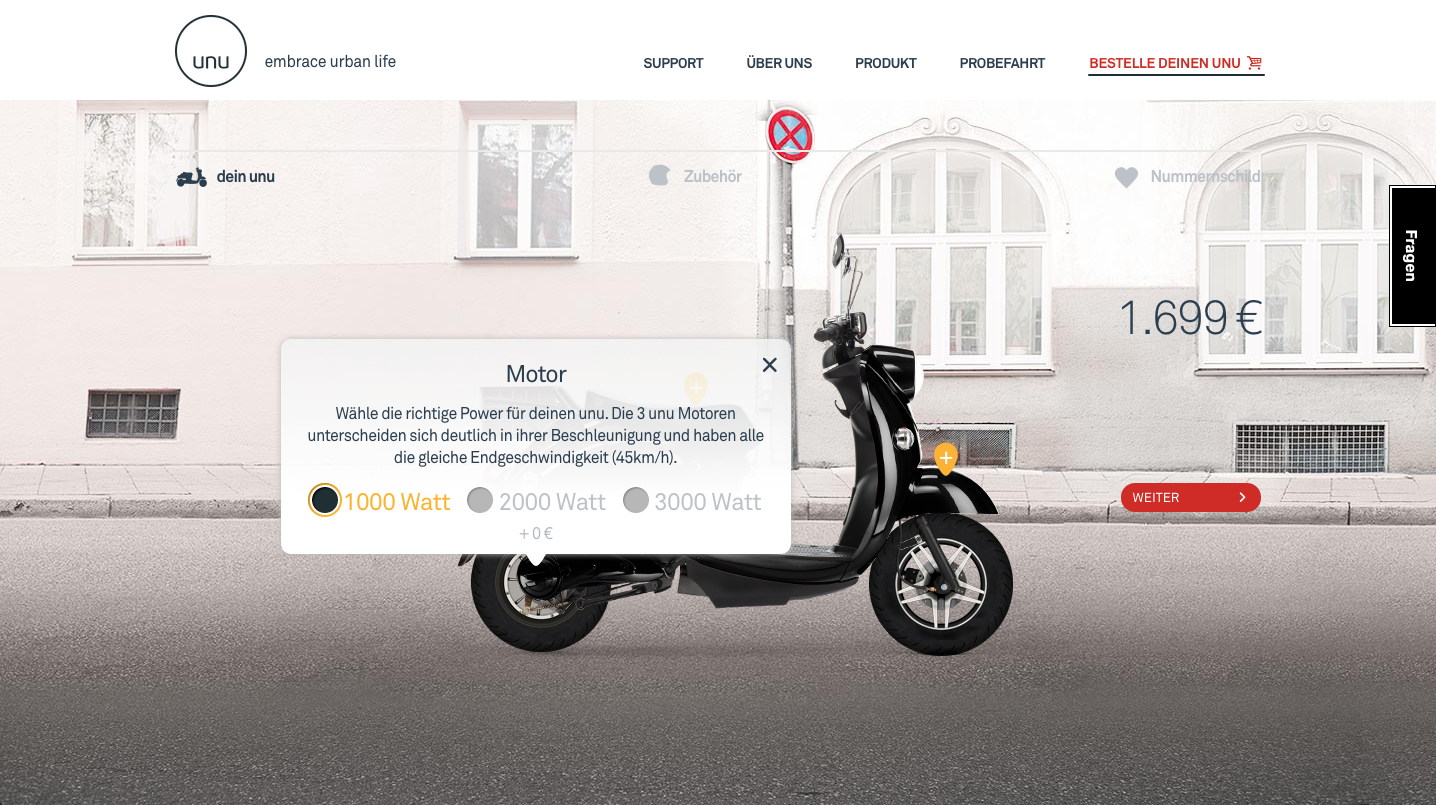
\includegraphics[width=\linewidth]{RelatedWork/img/unu-config.png}
  \caption{UNU GmbH\copyright{} electric scooter web configurator\cite{unu:2015:Online}}
\label{fig:unu-config}
\end{minipage}
\begin{minipage}{.45\textwidth}
\centering
  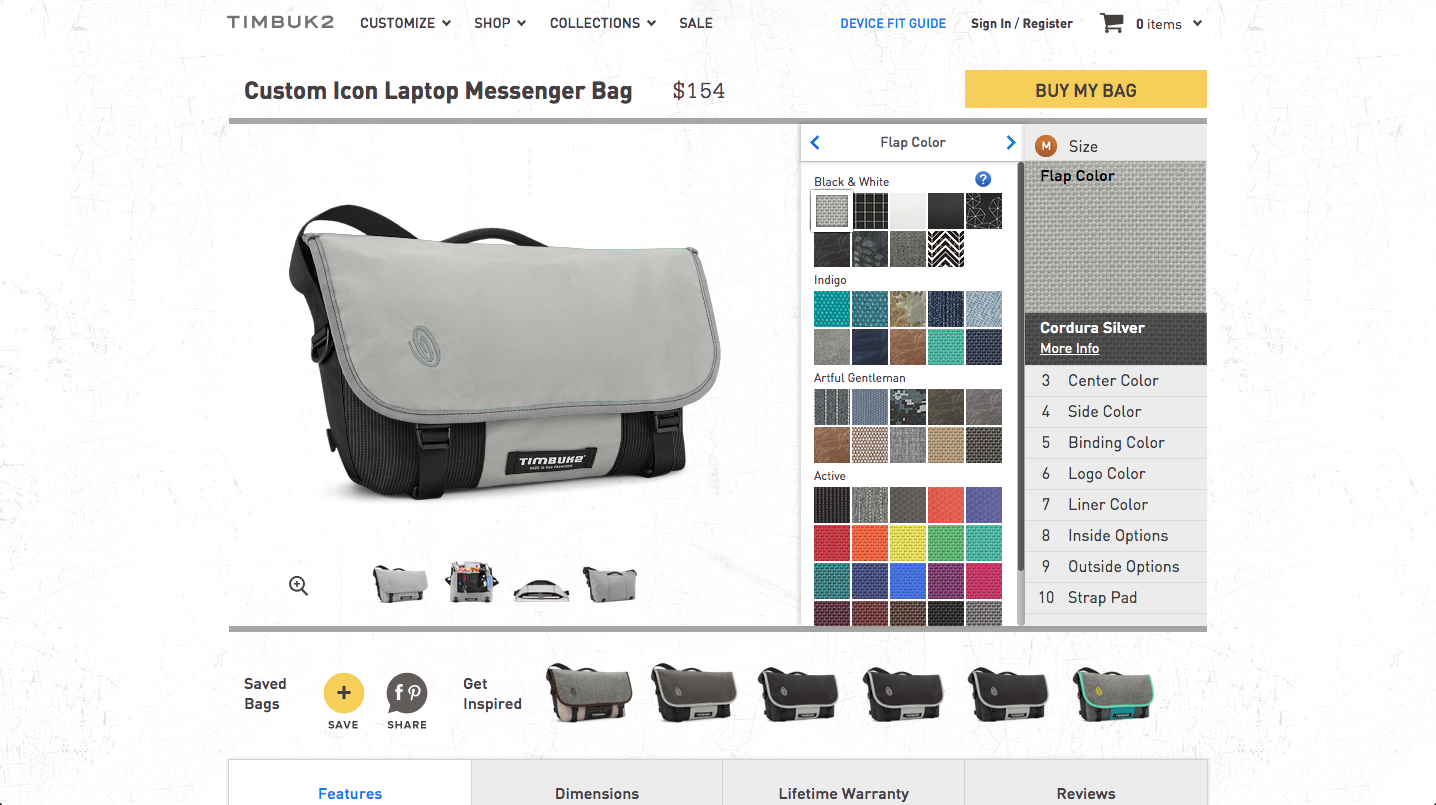
\includegraphics[width=\linewidth]{RelatedWork/img/timbuk2-config.png}
  \caption{Timbuk2\copyright{} bag web configurator\cite{timbuk2:2015:Online}}
\label{fig:timbuk2-config}
\end{minipage}
\end{figure}

\subsubsection{Gates 3D Configurator}
As part of an action-research project from Living
Lab\cite{livinglabs:2015:Online} Rolland et al.\cite{rolland2012commerce}
developed a gate configurator for the French company Groupe Maine's gates. The
objective of the authors was to showcase the possibilities of 3D Web
technologies in e-commerce applications. The developed tool was build with the
Unitiy3D\cite{unity3d:2015:Online} game engine, a flexible tool principally
build for game development but it has proved to be also useful for architectural
visualization and graphic intense web applications. After a user has logged in
to the configurator, the platform allows customers to select from a variety of
gate styles visualized as 3D models placed on the right side controls (see fig.\ref{fig:gates-config}). The user has also the option of setting the environment in which the gate is being placed (left side controls). This can happen by either selecting a predefined environment of by uploading a picture of the user's home or place where the gate shall be installed later. Customers can position the gates in the uploaded photograph by operating dedicated slider controls. The main advantage of allowing customers to upload their own images is that this allows them to have a better idea of how the selected gates will look in the final environment making them feel more comfortable about their decision. The authors state that they preferred the superimposition of a custom image rather than letting the user customize the environment with threes or buildings to make it look as close as possible because of the possible frame rate drop produced of handling many models and generating and because it is quite rare that somebody has a 3D model of his home. 

One of the main aspects of the gates configurator in respect to the research purposes the authors had, was that of developing a tool that improved the visualization of products with the end of encouraging the purchasing of the product in an online medium. To validate the design ideas behind the gate configurator and analyze the impact it had on customers, the authors performed an empirical evaluation. The results of the 27 evaluated participants showed that the manipulation of objects in 3D space seem naturally and was also confirmed to be important to the participants to have this option. This shows that having a realistic view of the product improves the chances of sale. 


\begin{figure}[hb]
\begin{center}
  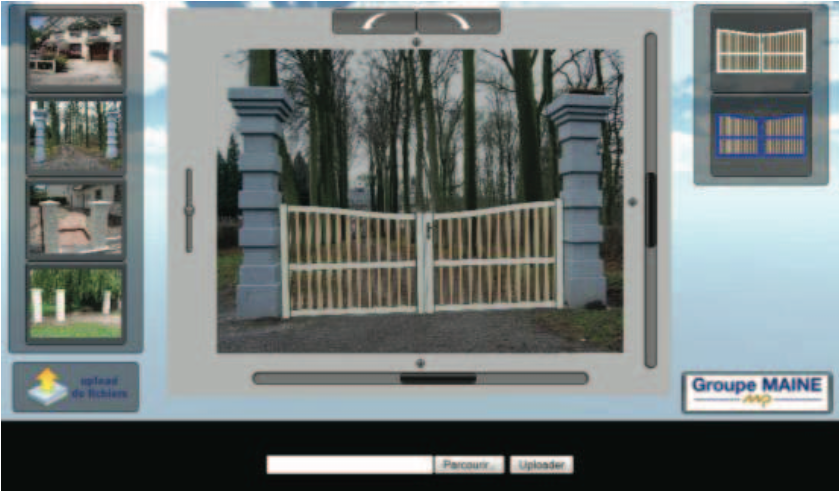
\includegraphics[width=.9\linewidth]{RelatedWork/img/gates-config.png}
  \caption{Groupe Maine's configurator\cite{rolland2012commerce} }
\label{fig:gates-config}
\end{center}
\end{figure}

\subsubsection{Makervis}

\subsubsection{Twikit}

\subsection{Activity Sculptures}

\subsubsection{Sweet Atoms}

\subsubsection{Mental Fabrications}

\subsection{Activity Data Sources}

\subsubsection{Fitness Tracker APIs}
\end{document}